% =======================
% B.Tech Final Year Project — End-Semester Thesis
% =======================
\documentclass[12pt,oneside]{report}

% -----------------------
% Packages
% -----------------------
\usepackage[
  a4paper,
  top=25mm,
  bottom=25mm,
  left=25mm,
  right=25mm,
  headsep=10mm,
  footskip=12mm
]{geometry}
\usepackage{array}
\usepackage{setspace}
\usepackage{graphicx}
\usepackage{booktabs}
\usepackage{tabularx}
\usepackage{tikz}
\usetikzlibrary{shapes, arrows, positioning}
\usepackage{tcolorbox}
\usepackage{array}
\usepackage{tabularx}
\usepackage{array}
\usepackage{multirow}
\usepackage{enumitem}
\usepackage{titlesec}
\usepackage{fancyhdr}
\usepackage{hyperref}
\usepackage{tocloft}
\usepackage{pdflscape}     % landscape pages with correct PDF rotation
\usepackage{geometry}      % ensure header/footer areas are included
\usepackage{fancyhdr}
\geometry{includehead,includefoot}
\setlength{\headheight}{14pt} % avoid fancyhdr warnings

\usepackage{csquotes}
\usepackage{float}
\usepackage{amsmath,amssymb}
\usepackage{siunitx}
\usepackage{newtxtext,newtxmath}
\usepackage{xcolor}
\usepackage{pdflscape}
\usepackage{caption}
\captionsetup{labelfont=bf}

% -----------------------
% Add header block for TOC / LOF / LOT
% -----------------------
% Tighter dot leaders (optional)
\renewcommand{\cftdotsep}{1}

% Space around list titles (optional)
\setlength{\cftbeforetoctitleskip}{0pt}
\setlength{\cftaftertoctitleskip}{12pt}
\setlength{\cftbeforeloftitleskip}{0pt}
\setlength{\cftafterloftitleskip}{12pt}
\setlength{\cftbeforelottitleskip}{0pt}
\setlength{\cftafterlottitleskip}{12pt}

% Make number columns wide enough for multi-digits
\renewcommand{\cftsecnumwidth}{3.0em}
\renewcommand{\cftsubsecnumwidth}{4.0em}
\renewcommand{\cftfignumwidth}{3.2em}
\renewcommand{\cfttabnumwidth}{3.2em}

% (Optional) tighten some spacing
\setlength{\cftbeforesecskip}{0pt}
\setlength{\cftparskip}{0pt}

% Macro for one-line header
\newcommand{\ListHeader}[3]{%
  \par\vspace{0.3\baselineskip}%
  \noindent\begin{tabular*}{\textwidth}{@{\extracolsep{\fill}}lll}
    \textbf{#1} & \textbf{#2} & \textbf{#3}
  \end{tabular*}\par
  \vspace{0.25\baselineskip}\hrule\vspace{0.5\baselineskip}%
}

% Hook header after list titles
\renewcommand{\cftaftertoctitle}{%
  \ListHeader{Chapter / Section}{Title / Description}{Page}%
}
\renewcommand{\cftafterloftitle}{%
  \ListHeader{Figure No.}{Caption / Description}{Page}%
}
\renewcommand{\cftafterlottitle}{%
  \ListHeader{Table No.}{Caption / Description}{Page}%
}

% (Optional) make list titles bold / bigger
\renewcommand{\cfttoctitlefont}{\bfseries\Large}
\renewcommand{\cftloftitlefont}{\bfseries\Large}
\renewcommand{\cftlottitlefont}{\bfseries\Large}

% -----------------------
% Bibliography setup
% -----------------------
\usepackage[backend=biber,style=ieee,sorting=none]{biblatex}
\addbibresource{references.bib}

% -----------------------
% Paragraph formatting to match guideline 4.3
% -----------------------
\setlength{\parindent}{3em}
\setlength{\parskip}{6pt}
\titlespacing*{\section}{0pt}{*2}{12pt}
\titlespacing*{\subsection}{0pt}{*1.5}{12pt}
\clubpenalty=10000
\widowpenalty=10000
\displaywidowpenalty=10000

% -----------------------
% Other Formatting
% -----------------------
\onehalfspacing

% Chapter heading format
\titleformat{\chapter}[display]
  {\bfseries\large\raggedleft}
  {\MakeUppercase{CHAPTER}\\[0.25em]{\fontsize{36}{40}\selectfont\thechapter}}
  {0.75em}
  {\bfseries\LARGE}
\titlespacing*{\chapter}{0pt}{-1em}{1.25em}

\titleformat{\section}{\bfseries\large}{\thesection}{0.6em}{}
\titleformat{\subsection}{\bfseries}{\thesubsection}{0.6em}{}

% Headers/footers
\pagestyle{fancy}
\fancyhf{}
\fancyhead[L]{\leftmark}
\fancyfoot[C]{\thepage}
\renewcommand{\headrulewidth}{0pt}
\renewcommand{\footrulewidth}{0pt}

% Hyperref setup
\hypersetup{
  colorlinks=true, linkcolor=blue, citecolor=blue, urlcolor=blue,
  pdftitle={B.Tech End-Sem Thesis}, pdfauthor={Swarup Chanda et al.}
}

% -----------------------
% Meta information
% -----------------------
\newcommand{\ThesisTitle}{\textbf{Speech-to-speech Translation with Personalized Voice and Synchronized Lip Movement}}
\newcommand{\Programme}{B.Tech in Computer Science and Engineering}
\newcommand{\Department}{Department of Computer Science and Engineering}
\newcommand{\Institute}{National Institute of Technology Silchar}
\newcommand{\SupervisorName}{Dr. Partha Pakray}
\newcommand{\SubmissionMonth}{December}
\newcommand{\SubmissionYear}{2025}
\newcommand{\GroupNumber}{18}

\newcommand{\MemberA}{Swarup Chanda}
\newcommand{\RegA}{2212170}
\newcommand{\MemberB}{Mahesh Birajdar}
\newcommand{\RegB}{2212124}
\newcommand{\MemberC}{Vyshnavi Chilaka}
\newcommand{\RegC}{2212004}
\newcommand{\MemberD}{Ayush Mani Roy}
\newcommand{\RegD}{2212183}
\newcommand{\MemberE}{Asad Ahmed}
\newcommand{\RegE}{2212166}



% -----------------------
% Title Page
% -----------------------
\begin{document}
\begin{titlepage}
  \centering

  {\Large \textbf{SPEECH TO SPEECH TRANSLATION  \\ WITH PERSONALIZED VOICE \\ AND SYNCHRONIZED LIP MOVEMENT}\\[1.2em]}

  {A Report Submitted in\\[0.15em]
  Partial Fulfillment of the Requirements for the Degree of\\[0.25em]
  \textbf{\Programme}\\[3.0em]}

  {\large \textbf{Project Group No.: \GroupNumber}\\[1.0em]}

  \noindent
  \textbf{Team Members:}\\[0.5em]
  \MemberA\ (\RegA)\\
  \MemberB\ (\RegB)\\
  \MemberC\ (\RegC)\\
  \MemberD\ (\RegD)\\ 
  \MemberE\ (\RegE)\\ [2.0em]

  \begin{center}
    {\textbf{Under the Supervision of}\\[0.3em]
    \SupervisorName\\
    Associate Professor, Department of Computer Science and Engineering\\
    \Institute\\[2.0em]}
  \end{center}

  \IfFileExists{NIT_Silchar_logo.png}{\includegraphics[width=0.18\textwidth]{NIT_Silchar_logo.png}}{\vspace{0.5em}}\\[1.0em]

  {\large \Department\\[0.5em]
  \textbf{NATIONAL INSTITUTE OF TECHNOLOGY SILCHAR}\\[0.5em]
  \SubmissionMonth~\SubmissionYear}

  \vfill
\end{titlepage}

% -----------------------
% Declaration (group wording)
% -----------------------
\thispagestyle{empty}
\begin{center}
  {\LARGE \textbf{DECLARATION}}\\[1.5em]
\end{center}
\noindent
Report Title: Speech-to-speech Translation with Personalized Voice and Synchronized Lip Movement \\
Degree for which the Report is submitted: B.Tech. in Computer Science and Engineering\\[1.2em]
I hereby declare that the work presented in this report is the result of my own effort and has not been submitted elsewhere for any degree or diploma. Where the ideas or words of others have been used, they have been duly acknowledged and cited in the reference section.
This report has been prepared without any form of plagiarism and adheres to the principles of academic honesty and integrity. No falsified or fabricated data have been included. I understand that any violation of these principles may lead to disciplinary action by the Institute, including withdrawal of the degree awarded.\\[2.5em]


\noindent\begin{tabular}{p{8.5cm}p{5cm}}
\MemberA\ (\RegA) & \rule{5cm}{0.4pt} \\[1.5em]
\MemberB\ (\RegB) & \rule{5cm}{0.4pt} \\[1.5em]
\MemberC\ (\RegC) & \rule{5cm}{0.4pt} \\[1.5em]
\MemberD\ (\RegD) & \rule{5cm}{0.4pt} \\[1.5em]
\MemberE\ (\RegE) & \rule{5cm}{0.4pt} \\[1.5em]
\end{tabular}

\newpage

% -----------------------
% Certificate (group wording)
% -----------------------
\thispagestyle{empty}
\begin{center}
  {\LARGE \textbf{CERTIFICATE}}\\[1.5em]
\end{center}
\noindent

This is to certify that the Final Year Project report entitled \emph{\ThesisTitle}, submitted by \textbf{Project Group \GroupNumber{}} (Members: \MemberA{} [\RegA], \MemberB{} [\RegB], \MemberC{} [\RegC], and \MemberD{} [\RegD]) in partial fulfillment of the requirements for the award of the degree of \Programme{} at \Institute{}, is a genuine and bonafide record of the research work carried out by the aforementioned students under my supervision and guidance. 

The results presented in this report are based on the students’ independent efforts, carried out in the Department of  Computer Science and Engineering, during the academic session 2025–26. This work has not been submitted elsewhere, either wholly or partially, for any other degree or diploma.\\[5em]
\noindent
\rule{0.35\linewidth}{0.4pt}\\
\textbf{Supervisor}\\
\SupervisorName\\
Associate Professor, Department of Computer Science and Engineering\\
National Institute of Technology Silchar\\[4.0em]
\noindent Date: \rule{0.25\linewidth}{0.4pt} 

\newpage


% -----------------------
% Acknowledgments & Abstract
% -----------------------
\pagenumbering{roman}
\setcounter{page}{1}
\chapter*{Acknowledgments}

{
We express our sincere gratitude to our supervisor, \SupervisorName, Associate Professor, Department of Computer Science and Engineering, \Institute, for his invaluable guidance, constant encouragement, and insightful suggestions throughout the course of this project. His mentorship has played a pivotal role in deepening our understanding of the subject and in successfully completing this End-Semester Final Year Project Report.

We are profoundly thankful to all the faculty members and technical staff of the \Department{} for their continuous support and valuable insights. We also extend special thanks to Virtual Machine under \SupervisorName,  for providing the essential facilities, resources, and technical computing power that greatly aided the experimental and analytical components of this study.

Finally, we would like to convey our heartfelt appreciation to our peers and teammates for their cooperation, constructive discussions, and unwavering enthusiasm, which have contributed immensely to the successful completion of this work.
}\\[2.5em]


\newpage

\chapter*{Abstract}

Speech-to-speech translation (S2ST) has emerged as a transformative area of research, primarily driven by the need for seamless multilingual communication, accessibility, and natural human--computer interaction. This project presents an end-to-end speech-to-speech translation system with personalized voice cloning and synchronized lip movement, specifically designed for Indian accent based languages.

The proposed system integrates four major components: (1) OpenAI Whisper~\cite{radford2023whisper} for automatic speech recognition (ASR), (2) IndicTrans2~\cite{gala2023indictrans2} for machine translation across various major Indian languages, (3) Cutomized IndicF5~\cite{indicf5_2025} Model for personalized voice cloning that preserves the speaker's identity and accent, and (4) MuseTalk~\cite{zhang2023musetalk} 1.5 personalized trained model for Indian accent based real-time lip synchronization. The unified pipeline enables applications such as multilingual video dubbing, inclusive education tools, personalized virtual assistants, and accessibility systems.

Evaluation results demonstrate high performance across all modules: Whisper~\cite{radford2023whisper} ASR achieves a Word Error Rate (WER) of 1.29\% and Character Error Rate (CER) of 2.35\%; voice cloning achieves cosine similarity of approximately 0.92 with strong accent preservation; and lip synchronization achieves LSE-C of 0.2557 and FID of 23.67. Human evaluation yields Mean Opinion Scores (MOS) of 4.01+ for audio quality and 3.98 for lip-sync realism.

This work represents a significant step toward natural, multilingual AI communication systems that preserve human identity, clarity, and realism.

\textbf{Keywords:} Speech-to-Speech Translation, Voice Cloning, Lip Synchronization, Whisper~\cite{radford2023whisper} ASR, IndicTrans2~\cite{gala2023indictrans2}, IndicF5~\cite{indicf5_2025}, MuseTalk~\cite{zhang2023musetalk}1.5, Indian Languages, Multilingual AI

\newpage

% -----------------------
% TOC / LOF / LOT
% -----------------------

\tableofcontents
\newpage
\listoffigures
\newpage
\listoftables
\newpage
\chapter*{Glossary of Symbols, Abbreviations, and Notations}
\label{ch:glossary}
\section*{A. Symbols and Notations}

\begin{table}[H]
\centering
\caption{Primary symbols and definitions used in this study.}
\label{tab:symbols}
\renewcommand{\arraystretch}{1.05}
\setlength{\tabcolsep}{4.5pt}
\small
\begin{tabular}{@{}ll@{}}
\toprule
\textbf{Symbol} & \textbf{Description} \\
\midrule
$X$ & Input audio signal \\
$Y$ & Output text sequence (ASR) \\
$S$ & Source language text \\
$T$ & Target language text (translated) \\
$P(Y|X)$ & Conditional probability of text given audio \\
$f_{\theta}$ & Translation model with parameters $\theta$ \\
$g_{\phi}$ & Voice synthesis model with parameters $\phi$ \\
$\hat{M}$ & Reconstructed mel-spectrogram \\
$e_s$ & Speaker embedding vector \\
$A$ & Audio features for lip-sync \\
$V$ & Video frames for lip-sync \\
$\psi$ & Lip synchronization mapping function \\
$y_t$ & Output token at time step $t$ \\
$y_{<t}$ & Output tokens before time step $t$ \\
$t_j$ & Target token at position $j$ (translation) \\
$I_t^o$ & Output (generated) video frame at time $t$ \\
$I_t^{gt}$ & Ground truth video frame at time $t$ \\
$\mathcal{L}_{rec}$ & Reconstruction loss (L1 norm) \\
$\mathcal{L}_p$ & Perceptual loss (VGG19-based) \\
$\mathcal{L}_{sync}$ & Lip synchronization loss \\
$\mathcal{L}_{GAN}$ & Adversarial (GAN) loss \\
$\mathcal{V}$ & VGG19 feature extractor \\
$D$ & Discriminator network \\
$A_{mel}$ & Mel-spectrogram audio features \\
$A_{ref}$ & Reference audio for voice cloning \\
$T_{ref}$ & Reference transcript for voice cloning \\
$\mathcal{E}$ & Speaker encoder function \\
\bottomrule
\end{tabular}
\end{table}

\newpage
\section*{B. Abbreviations and Full Forms}

\begin{table}[H]
\centering
\caption{Abbreviations used in the Report.}
\label{tab:abbrev}
\renewcommand{\arraystretch}{1.05}
\setlength{\tabcolsep}{4.5pt}
\small
\begin{tabular}{@{}ll@{}}
\toprule
\textbf{Abbreviation} & \textbf{Full Form} \\
\midrule
AI & Artificial Intelligence \\
ASR & Automatic Speech Recognition \\
BLEU & Bilingual Evaluation Understudy \\
CER & Character Error Rate \\
FID & Fréchet Inception Distance \\
LSE-C & Lip Sync Error - Confidence \\
MOS & Mean Opinion Score \\
MT & Machine Translation \\
NLP & Natural Language Processing \\
S2ST & Speech-to-Speech Translation \\
STT & Speech-to-Text \\
TTS & Text-to-Speech \\
WER & Word Error Rate \\
GPU & Graphics Processing Unit \\
API & Application Programming Interface \\
DNN & Deep Neural Network \\
RNN & Recurrent Neural Network \\
LSTM & Long Short-Term Memory \\
GAN & Generative Adversarial Network \\
VAE & Variational Autoencoder \\
\bottomrule
\end{tabular}
\end{table}

\pagenumbering{arabic}

% =====================================================
% REQUIRED SECTIONS (a)–(f)
% =====================================================

\chapter{Introduction}
\label{ch:intro}

\section{Background of the Scenario}

Speech-to-speech translation (S2ST) has emerged as a transformative area of research, primarily driven by the need for seamless multilingual communication, accessibility, and natural human-computer interaction. Traditional translation systems rely heavily on text-based methods, where speech is first converted into text, then translated, and finally synthesized back into speech. However, these pipelines often fail to preserve the speaker's identity, emotional tone, accent, and timing elements critical for natural and human-like communication.

In multilingual countries like India, where more than 22 major languages and hundreds of dialects coexist, building a translation system that preserves originality and identity becomes essential. Users expect systems that do more than just translate they expect continuity of voice, personality, and authenticity across languages. Furthermore, the rise of digital assistants, remote classrooms, and AI-driven content creation has created demand for tightly synchronized visual and auditory outputs, especially lip movement aligned with speech.

This project aims to address these gaps by integrating speech recognition, translation, high-quality voice cloning, and real-time lip synchronization into a unified system. The work builds upon recent advancements in Whisper~\cite{radford2023whisper} ASR, IndicTrans2~\cite{gala2023indictrans2} translation, IndicF5~\cite{indicf5_2025} voice cloning, and MuseTalk~\cite{zhang2023musetalk}-based lip-motion synthesis, creating a pipeline capable of converting speech from one language to another while maintaining the same personalized voice and synchronized facial movement.

This integrated pipeline enables a wide range of impactful real-world applications:

\begin{itemize}
    \item \textbf{Multilingual video dubbing:}  
    The system can automatically translate and re-synthesize speech while preserving the speaker’s identity, producing lip-synchronized videos suitable for films, lectures, interviews, and social media content across different languages.

    \item \textbf{Inclusive education platforms:}  
    By removing language barriers, the pipeline allows academic lectures, tutorials, and training modules to be delivered in multiple languages, making high-quality learning resources accessible to students from diverse linguistic backgrounds.

    \item \textbf{Personalized virtual assistants:}  
    Assistant systems can adopt the user’s own cloned voice or provide natural localized speech output, creating more relatable, culturally adaptive, and user-friendly AI interaction experiences.

    \item \textbf{Accessibility solutions for hearing-impaired and speech-impaired individuals:}  
    The model can convert spoken audio to synchronized, visually articulated content, aiding comprehension. Additionally, voice cloning enables individuals with vocal impairment to restore a version of their own natural voice.

    \item \textbf{Real-time communication aids:}  
    The pipeline can be adapted for live translation scenarios, enabling conversations between speakers of different languages with near-real-time lip-synced video and personalized speech output.
\end{itemize}

\section{Closure}

The proposed system demonstrates the feasibility of a unified, end-to-end framework that integrates speech recognition, translation, voice cloning, and lip-synchronization into a coherent workflow. By preserving speaker identity and ensuring natural audiovisual alignment, the pipeline provides a robust foundation for next-generation human–computer interaction and multilingual communication technologies. The modular nature of the framework allows further extensions—such as real-time deployment, enhanced emotion modeling, or domain-specific fine-tuning—making it a promising direction for future research and practical applications.





\chapter{Literature Review}
\label{ch:lit}

\section{Summary of the Literature Review}

The literature on speech-to-speech translation (S2ST) spans multiple key domains: Automatic Speech Recognition (ASR), Machine Translation (MT), Text-to-Speech (TTS), and modern lip synchronization techniques.

\subsection{Speech Recognition (ASR)}

OpenAI Whisper~\cite{radford2023whisper} represents one of the most robust and multilingual ASR systems available today. Trained on 680,000 hours of multilingual and multitask supervised data collected from the web, Whisper~\cite{radford2023whisper} demonstrates remarkable ability to handle non-native accents, noisy audio, and multilingual input. Its encoder-decoder transformer architecture makes it well-suited for Indian linguistic diversity, where speakers often code-switch between languages and exhibit unique prosodic patterns.The architecture follows the standard multi-head attention mechanism introduced in~\cite{vaswani2017attention}.

\subsection{Machine Translation}

IndicTrans2~\cite{gala2023indictrans2}, developed by AI4Bharat, represents the first open-source transformer-based multilingual Neural Machine Translation (NMT) model that supports high-quality translations across all 22 scheduled Indic languages.The translation stage adopts the transformer encoder–decoder architecture~\cite{vaswani2017attention} implemented within IndicTrans2~\cite{gala2023indictrans2}. The model adopts script unification wherever feasible to leverage transfer learning through lexical sharing between languages. Overall, the model supports five scripts: Perso-Arabic (Kashmiri, Sindhi, Urdu), Ol Chiki (Santali), Meitei (Manipuri), Latin (English), and Devanagari (used for all remaining languages).

The model is trained on the Bharat Parallel Corpus Collection (BPCC), a comprehensive parallel corpus comprising approximately 230 million bitext pairs. BPCC consists of two components:
\begin{itemize}
    \item \textbf{BPCC-Mined:} Contains approximately 228 million pairs, including 126 million newly added pairs.
    \item \textbf{BPCC-Human:} Comprises 2.2 million gold standard English-Indic pairs, with additional subsets for Wikipedia sentences (BPCC-H-Wiki, 644K pairs) and everyday use cases (BPCC-H-Daily, 139K pairs).
\end{itemize}

For evaluation, the IN22 test set provides a comprehensive benchmark for multi-domain, n-way parallel translation assessment across 22 Indic languages. The benchmark includes IN22-Gen (combining Wikipedia and web sources with 1024 sentences) and IN22-Conv (conversational domain with 1503 sentences). The model achieves state-of-the-art performance using chrF++ as the primary metric, along with BLEU and COMET scores.

In our implementation, we utilize IndicTrans2~\cite{gala2023indictrans2} for translation to six major Indian languages: Hindi (hin\_Deva), Bengali (ben\_Beng), Assamese (asm\_Beng), Marathi (mar\_Deva), Tamil (tam\_Taml), and Telugu (tel\_Telu).

\subsection{Voice Cloning and Speaker Modeling}

Voice cloning research is dominated by encoder-decoder TTS models that aim to capture and reproduce speaker-specific characteristics. Recent advances in this field include:
\begin{itemize}
    \item Transfer Learning from Speaker Verification to TTS
    \item Zero-shot voice cloning using speaker embeddings
    \item Few-shot speaker adaptation techniques
\end{itemize}

\subsubsection{IndicF5: High-Quality Text-to-Speech for Indian Languages}

IndicF5~\cite{indicf5_2025} is a near-human polyglot Text-to-Speech (TTS) model developed by AI4Bharat, trained on 1,417 hours of high-quality speech data from multiple sources including Rasa, Indic-TTS foundation model~\cite{kumar2023indictts}, LIMMITS, and IndicVoices-R datasets. The model supports 11 Indian languages: Assamese, Bengali, Gujarati, Hindi, Kannada, Malayalam, Marathi, Odia, Punjabi, Tamil, and Telugu.

The key innovation of IndicF5~\cite{indicf5_2025} lies in its reference-based synthesis approach, which requires three inputs for speech generation:
\begin{enumerate}
    \item \textbf{Text to synthesize:} The content to be converted to speech.
    \item \textbf{Reference prompt audio:} An example speech clip that guides prosody and speaker characteristics.
    \item \textbf{Reference transcript:} The text spoken in the reference audio.
\end{enumerate}

This architecture enables zero-shot~\cite{jia2018transfer, indicf5_2025} voice cloning, where the model can replicate a speaker's voice characteristics from a short audio sample without requiring speaker-specific fine-tuning.

\subsubsection{AI4Bharat Indic-TTS Foundation}

The foundational work for Indian language TTS was established through the AI4Bharat Indic-TTS project, which systematically evaluated acoustic models, vocoders, supplementary loss functions, and training schedules for Dravidian and Indo-Aryan languages. The research identified that monolingual models using FastPitch acoustic model combined with HiFi-GAN V1 vocoder, trained jointly on male and female speakers, achieve optimal performance.

The unified TTS architecture consists of:
\begin{itemize}
    \item \textbf{Acoustic Model (FastPitch):} Generates mel-spectrograms from input text with pitch prediction.
    \item \textbf{Vocoder (HiFi-GAN V1):} Converts mel-spectrograms to high-fidelity audio waveforms.
\end{itemize}

This architecture provides SOTA performance across 13 Indian languages as measured by Mean Opinion Scores (MOS), significantly improving upon existing models.

\subsection{Lip-Synchronization Techniques}

Earlier lip-sync systems such as Wav2Lip~\cite{prajwal2020lipsync}, viseme-based systems~\cite{hoon2015viseme} and SyncNet rely purely on audio--visual frame-level alignment but fail in producing natural facial transitions and handling edge cases. Recent work has explored disentangling lip-motion information from audio~\cite{wang2022lipdisentangle}. MuseTalk~\cite{zhang2023musetalk} introduces significant improvements including:
\begin{itemize}
    \item Latent-space editing for smoother transitions
    \item Face-aware dynamics that preserve identity
    \item High-quality motion synthesis
\end{itemize}

These advancements allow real-time generation of realistic lip movement that maintains temporal consistency with the audio.
\section{Research Gap Evaluation}

Despite significant progress in speech translation, voice cloning, and lip-synchronization technologies, several unresolved challenges continue to hinder the development of a unified, natural, and real-time Audio-Visual Speech-to-Speech Translation (AV-S2ST) system. A detailed evaluation of these research gaps is presented below:

\begin{enumerate}
    \item \textbf{Insufficient preservation of speaker identity across languages.}  
    Current cascaded S2ST systems rely on generic TTS models that fail to maintain the speaker’s unique timbre, prosody, and vocal style after translation.Direct S2ST has been explored through models such as Translatotron~\cite{jia2019translatotron}, discrete unit S2ST~\cite{lee2022discrete_s2st}, and cascade vs direct studies~\cite{freitag2022cascade}. Direct S2ST models partially address this but remain unstable and require large paired datasets, resulting in translated speech that sounds disconnected from the original speaker.

    \item \textbf{Limited training on Indian accents and low-resource languages.}  
    Most ASR, MT, and TTS models are trained on high-resource Western languages, leading to degraded performance for Indian languages with diverse phonetic structures. This results in unnatural prosody, pronunciation errors, and reduced speaker similarity in cloned voices for Indian users.

    \item \textbf{Inaccuracies in multilingual audio--visual synchronization.}  
    Lip-sync systems often struggle with Indian phonemes and rapid articulatory transitions, creating subtle but noticeable mismatches between lip movements and synthesized speech. These errors reduce realism and risk pushing the output into the ``uncanny valley.''

    \item \textbf{Fragmented architecture across independent modules.}  
    ASR, translation, TTS, voice cloning, and lip-sync models typically operate as isolated components. This fragmentation increases error propagation, computational latency, and manual coordination requirements, highlighting the absence of a unified, end-to-end AV-S2ST pipeline.

    \item \textbf{Scarcity of large-scale Indian datasets for voice cloning and lip-sync.}  
    India lacks extensive multimodal corpora covering diverse accents, expressions, and speaker identities. The lack of audio--text--video datasets limits the training and benchmarking of generative models optimized for Indian demographics.

    \item \textbf{Inability to achieve real-time performance in end-to-end systems.}  
    Cascaded systems accumulate latency across ASR--MT--TTS modules, while direct S2ST models demand high computational resources. Achieving real-time translation, synthesis, and video rendering remains a major challenge for practical deployment.

    \item \textbf{Weak prosody and emotion transfer during translation and synthesis.}  
    The ``text bottleneck'' in cascaded pipelines suppresses emotional cues, resulting in flat or emotionally inaccurate speech that fails to preserve the expressiveness of the original speaker.

    \item \textbf{Ethical and security vulnerabilities due to deepfake risks.}  
    Highly realistic voice cloning and lip-synchronization raise concerns related to impersonation, misinformation, fraud, and non-consensual content. Current systems lack integrated watermarking, authentication, and deepfake detection mechanisms.

    \item \textbf{Absence of unified evaluation metrics for multimodal dubbing quality.}  
    While individual modules have established metrics (WER for ASR, BLEU for MT, MOS for TTS, LSE for lip-sync), there is no single composite metric to evaluate the holistic quality of audio--visual dubbing systems.

    \item \textbf{Limited personalization and user adaptability.}  
    Existing systems rarely support personalized lip-motion generation approaches like StyleLipSync~\cite{kimin2023stylelipsync} explore style-conditioned synthesis. voice behavior, adaptive prosody modeling, or user-specific emotion transfer. This limits the potential for highly customized dubbing and accessibility applications.
\end{enumerate}


This research aims to bridge these gaps by developing an integrated system that addresses each of these limitations.

\section{Objectives of the Present Work}

The primary objectives of this project are:

\begin{enumerate}
    \item \textbf{To collect, preprocess, and prepare multilingual audio--text datasets} suitable for Indian languages by performing noise reduction, normalization, segmentation, and feature extraction to ensure high-quality inputs for downstream models.

    \item \textbf{To develop a speech-to-speech translation pipeline} that converts spoken language into six major Indian languages while preserving linguistic context, fluency, and expressive meaning.

    \item \textbf{To generate translated speech using a personalized cloned voice} through the IndicF5~\cite{indicf5_2025} model, ensuring that the speaker’s unique vocal identity timbre, pitch, and speaking style is preserved across all target languages.

    \item \textbf{To produce lip-synchronized output videos} using MuseTalk~\cite{zhang2023musetalk}~1.5 by aligning translated audio with realistic facial articulation, enhancing immersion and visual naturalness.

    \item \textbf{To integrate all individual models into a unified, end-to-end pipeline} and fine-tune key parameters to improve system accuracy, robustness, and real-time operability.

    \item \textbf{To design a user-friendly web interface} enabling users to record, translate, generate cloned speech, and view synchronized lip animations within an accessible application.

    \item \textbf{To evaluate the complete system using objective and subjective metrics} including WER (ASR accuracy), BLEU (translation quality), MOS (speech naturalness), Speaker Similarity, LSE-C/LSE-D (lip-sync accuracy), FID/SSIM (visual quality), and human evaluation.
\end{enumerate}


\section{Closure}

This chapter summarized the theoretical background, existing technologies, and research gaps in the domain of speech-to-speech translation. The next chapter describes the methodology and integrated architecture of the proposed system.

\chapter{Methodology}
\label{ch:method}

\section{Introduction}

The proposed methodology follows a modular and systematic design, enabling the transformation of spoken content from one language to another while preserving the speaker’s vocal identity and achieving realistic lip synchronization. The framework integrates four state-of-the-art deep learning components, Automatic Speech Recognition (ASR), Neural Machine Translation (NMT), Voice Cloning, and Lip-Sync Generation each optimized for a specific stage of the pipeline. By decomposing the overall task into sequential and interdependent modules, the system ensures robustness, interpretability, and scalability across diverse linguistic and visual domains. The outputs produced at each stage are carefully structured to serve as high-quality inputs to the subsequent components, forming a smooth end-to-end workflow.

\section{System Overview}

The methodology consists of four major components operating in a cascaded pipeline:

\begin{enumerate}
    \item \textbf{Speech-to-Text (ASR):} Converting input audio to text using Whisper~\cite{radford2023whisper}.
    \item \textbf{Machine Translation:} Translating text to the target language using IndicTrans2~\cite{gala2023indictrans2}.
    \item \textbf{Voice Cloning (TTS):} Synthesizing translated text in a cloned version of the speaker’s voice using IndicF5~\cite{indicf5_2025}.
    \item \textbf{Lip Synchronization:} Generating synchronized video output using MuseTalk~\cite{zhang2023musetalk}~1.5.
\end{enumerate}

Each module processes its input and forwards a structured output to the next stage, enabling a fully automated pipeline from the raw input video to the final translated, voice-cloned, and lip-synced video.




\section{Physical Modelling}

Physical modeling in this context represents the real-world interaction of multiple signal domains:

\begin{itemize}
    \item \textbf{Audio signals:} Time-domain waveforms captured from microphone input, typically sampled at 16 kHz for speech processing.
    \item \textbf{Text processing units:} Discrete token sequences representing linguistic content after ASR and before TTS.
    \item \textbf{Speaker timbre representation:} Embedding vectors that capture voice characteristics including pitch, tone, and speaking style.
    \item \textbf{Facial motion synthesis:} Frame-level visual features that represent lip positions, jaw movements, and facial expressions.
\end{itemize}

Signal models represent time-domain audio, mel spectrograms (frequency-time representations), and frame-aligned features for lip generation. The physical system must handle the temporal alignment between these different modalities while maintaining real-time processing capabilities.

\begin{figure}[H]
    \centering
    \includegraphics[width=0.9\textwidth]{spectrogram.png}
    \caption{Audio signal representations: (Top) Time-domain waveform showing amplitude variations over a 60-second audio sample; (Bottom) Corresponding mel spectrogram visualization displaying frequency content over time, which serves as input to the ASR and voice cloning modules.}
    \label{fig:spectrogram}
\end{figure}

\section{Mathematical Modelling}

The mathematical formulations underlying each component are as follows:

\subsection{Whisper ASR Model}

Whisper~\cite{radford2023whisper} is a transformer encoder--decoder model trained to map an input sequence of audio features $X$ (log-Mel spectrogram frames) to an output token sequence $Y = (y_1,\dots,y_T)$ representing the transcription. The conditional probability of the full transcription given the audio is factorized autoregressively as:
\begin{equation}
    P(Y \mid X)
    = \prod_{t=1}^{T} P\bigl(y_t \mid X, y_{<t}\bigr),
\end{equation}
where $y_{<t} = (y_1,\dots,y_{t-1})$ denotes all previously generated tokens.  
This formulation is \emph{correct} and corresponds to the standard sequence-to-sequence~\cite{radford2023whisper} modeling assumption.

The encoder transforms the input audio features $X$ into a sequence of hidden representations:
\begin{equation}
    H^{\mathrm{enc}} = \mathrm{Encoder}(X),
\end{equation}
where $H^{\mathrm{enc}} = (h^{\mathrm{enc}}_1,\dots,h^{\mathrm{enc}}_{L})$ and $L$ is the number of encoder time steps.

At each decoding step $t$, the decoder attends to the encoder states and the previously generated tokens $y_{<t}$ to produce a decoder hidden state:
\begin{equation}
    h^{\mathrm{dec}}_t = \mathrm{Decoder}\bigl(y_{<t}, H^{\mathrm{enc}}\bigr).
\end{equation}
The probability distribution over the next token is then obtained via a linear projection followed by a softmax:
\begin{equation}
    P\bigl(y_t = k \mid X, y_{<t}\bigr)
    = \mathrm{softmax}\!\left(W_o h^{\mathrm{dec}}_t + b_o\right)_k,
\end{equation}
where $W_o$ and $b_o$ are the output projection parameters and the subscript $k$ indexes the $k$-th token in the vocabulary.

During training, the parameters $\theta$ of the model are optimized by maximizing the log-likelihood of the ground-truth transcriptions, or equivalently by minimizing the negative log-likelihood (cross-entropy) loss:
\begin{equation}
    \mathcal{L}(\theta)
    = - \sum_{t=1}^{T} \log P_\theta\bigl(y_t^{\ast} \mid X, y_{<t}^{\ast}\bigr),
\end{equation}
where $y_t^{\ast}$ denotes the ground-truth token at position $t$. At inference time, the most likely sequence $\hat{Y}$ is obtained using beam search or greedy decoding:
\begin{equation}
    \hat{Y} = \arg\max_{Y} \; P(Y \mid X).
\end{equation}


\begin{figure}[H]
    \centering
    \includegraphics[width=0.85\textwidth]{speech_to_text_architecture.png}
    \caption{Speech-to-text and translation pipeline architecture showing audio extraction, Whisper~\cite{radford2023whisper} ASR engine for transcription, and IndicTrans NMT engine for multilingual translation to six major Indian languages (Assamese, Bengali, Hindi, Marathi, Odia, Tamil, and Telugu).}
    \label{fig:stt-architecture}
\end{figure}

Table~\ref{tab:bpcc-data} presents the composition of the BPCC training corpus used for IndicTrans2~\cite{gala2023indictrans2} model training.

\begin{table}[H]
\centering
\caption{Bharat Parallel Corpus Collection (BPCC) data composition for IndicTrans2~\cite{gala2023indictrans2} training.}
\label{tab:bpcc-data}
\renewcommand{\arraystretch}{1.1}
\begin{tabular}{@{}llr@{}}
\toprule
\textbf{Category} & \textbf{Source} & \textbf{Bitext Pairs} \\
\midrule
\multirow{4}{*}{BPCC-Mined} & Samanantar (Existing) & 19.4M \\
 & NLLB (Existing) & 85M \\
 & Samanantar++ (New) & 121.6M \\
 & Comparable (New) & 4.3M \\
\midrule
\multirow{4}{*}{BPCC-Human} & NLLB-Seed (Existing) & 18.5K \\
 & ILCI (Existing) & 1.3M \\
 & MASSIVE (Existing) & 115K \\
 & Wiki + Daily (New) & 783K \\
\midrule
\multicolumn{2}{l}{\textbf{Total}} & \textbf{$\approx$230M} \\
\bottomrule
\end{tabular}
\end{table}

\subsection{IndicTrans2 Translation Model}
The translation mapping is defined as:
\begin{equation}
T = f_{\theta}(S)
\end{equation}
where $S$ is the source language text, $T$ is the target language translation, and $\theta$ represents the model parameters.

IndicTrans2~\cite{gala2023indictrans2} employs a transformer-based encoder-decoder architecture with the following formulation for sequence-to-sequence translation:
\begin{equation}
P(T|S) = \prod_{j=1}^{|T|} P(t_j | t_{<j}, S; \theta)
\end{equation}
where $t_j$ represents the $j$-th token in the target sequence and $t_{<j}$ denotes all preceding target tokens.

The model utilizes script unification to enable cross-lingual transfer learning. For our implementation, the language codes follow the ISO 639-3 standard with script suffixes:
\begin{itemize}
    \item Hindi: \texttt{hin\_Deva} (Devanagari script)
    \item Bengali: \texttt{ben\_Beng} (Bengali script)
    \item Assamese: \texttt{asm\_Beng} (Bengali script)
    \item Marathi: \texttt{mar\_Deva} (Devanagari script)
    \item Tamil: \texttt{tam\_Taml} (Tamil script)
    \item Telugu: \texttt{tel\_Telu} (Telugu script)
\end{itemize}

The model supports both En-Indic and Indic-En translation directions, with inference optimized through CTranslate2 for efficient batch processing.

\subsection{IndicF5 Voice Cloning}
Voice cloning involves mel-spectrogram reconstruction conditioned on speaker embedding:
\begin{equation}
\hat{M} = g_{\phi}(T, e_s)
\end{equation}
where $\hat{M}$ is the synthesized mel-spectrogram, $T$ is the input text, $e_s$ is the speaker embedding, and $\phi$ represents the synthesis model parameters.

IndicF5~\cite{indicf5_2025} extends this formulation through a reference-based conditioning mechanism:
\begin{equation}
\hat{M} = g_{\phi}(T_{target}, \mathcal{E}(A_{ref}, T_{ref}))
\end{equation}
where $A_{ref}$ is the reference audio, $T_{ref}$ is the reference transcript, $T_{target}$ is the target text to synthesize, and $\mathcal{E}$ represents the speaker encoder that extracts prosodic and timbral characteristics.

The acoustic model builds on FastPitch~\cite{kim2021cvae}, while waveform reconstruction is performed by the HiFi-GAN vocoder, consistent with the Indic-TTS framework~\cite{kumar2023indictts}.
The acoustic model (FastPitch) generates mel-spectrograms with explicit pitch prediction:
\begin{equation}
\hat{M}, \hat{p} = \text{FastPitch}(T, e_s)
\end{equation}
where $\hat{p}$ represents the predicted pitch contour, enabling control over intonation patterns.

The vocoder (HiFi-GAN V1) then converts the mel-spectrogram to time-domain audio:
\begin{equation}
\hat{x} = \text{HiFi-GAN}(\hat{M})
\end{equation}
where $\hat{x}$ is the synthesized audio waveform at 24 kHz sampling rate.

The training objective for the TTS system combines multiple loss terms:
\begin{equation}
\mathcal{L}_{TTS} = \mathcal{L}_{mel} + \alpha \mathcal{L}_{pitch} + \beta \mathcal{L}_{duration}
\end{equation}
where $\mathcal{L}_{mel}$ is the mel-spectrogram reconstruction loss, $\mathcal{L}_{pitch}$ is the pitch prediction loss, and $\mathcal{L}_{duration}$ is the duration prediction loss.

\subsection{MuseTalk Lip Synchronization}
Lip synchronization is modeled as a latent-space mapping:
\begin{equation}
L = \psi(A, V)
\end{equation}
where $L$ represents the lip motion output, $A$ denotes audio features, $V$ represents video frames, and $\psi$ is the learned mapping function.

\begin{figure}[H]
    \centering
    \includegraphics[width=0.95\textwidth]{MuseTalk.jpg}
    \caption{MuseTalk~\cite{zhang2023musetalk} 1.5 architecture for lip synchronization. The model uses VAE encoders to extract latent features from reference and source images, combines them with Whisper~\cite{radford2023whisper}-encoded audio features, processes through a trainable Backbone UNet with audio attention, spatial convolution, and self-attention mechanisms, and finally decodes the predicted latent to generate the lip-synchronized output frame.}
    \label{fig:MuseTalk}
\end{figure}

\subsection{Lip Synchronization Loss Formulation}

The complete lip synchronization loss formulation, inspired by the MuseTalk~\cite{zhang2023musetalk} 1.5 methodology, combines reconstruction fidelity, perceptual similarity, adversarial quality enhancement, and synchronization accuracy.

\subsubsection{Reconstruction and Perceptual Losses}
The reconstruction loss based on the L1 norm ensures pixel-level fidelity between the generated output frame $I_t^o$ and the ground truth frame $I_t^{gt}$:
\begin{equation}
\mathcal{L}_{rec} = \| I_t^o - I_t^{gt} \|_1
\end{equation}

The perceptual loss uses VGG19 feature extraction layers to capture high-level semantic similarity:
\begin{equation}
\mathcal{L}_p = \| \mathcal{V}(I_t^o) - \mathcal{V}(I_t^{gt}) \|_2
\end{equation}
where $\mathcal{V}$ denotes the VGG19 feature extractor that maps images to a learned feature space.

\subsubsection{GAN Loss}
The adversarial training framework employs generator and discriminator losses to enhance visual realism. The generator loss is formulated as:
\begin{equation}
\mathcal{L}_G = \mathbb{E}[\log(1 - D(I_t^o))]
\end{equation}

The discriminator loss distinguishes between real and generated frames:
\begin{equation}
\mathcal{L}_D = \mathbb{E}[\log(1 - D(I_t^{gt}))] + \mathbb{E}[\log(D(I_t^o))]
\end{equation}

The combined GAN objective becomes:
\begin{equation}
\mathcal{L}_{GAN} = \mathcal{L}_G + \mathcal{L}_D
\end{equation}

\subsubsection{Lip-Sync Loss}
We incorporate the SyncNet-based lip synchronization formulation to ensure audio-visual alignment. The sync loss measures the probability that the generated lip movements match the corresponding audio mel-spectrogram features:
\begin{equation}
\mathcal{L}_{sync} = \frac{1}{N} \sum_{i=1}^{N} -\log\left[P_{sync}(syncnet(A_{mel}^i, I_t^i))\right]
\end{equation}
where $A_{mel}^i$ represents the mel-spectrogram audio features and $I_t^i$ denotes the corresponding video frame at time step $i$.

\subsubsection{Final Objective Function}
The weighted final loss combines all components with empirically determined coefficients:
\begin{equation}
\mathcal{L} = \mathcal{L}_{rec} + \lambda \mathcal{L}_p + \mu \mathcal{L}_{GAN} + \phi \mathcal{L}_{sync}
\end{equation}
where $\lambda = 0.01$, $\mu = 0.01$, and $\phi = 0.03$ in our implementation. These hyperparameters balance the contribution of each loss term to achieve optimal visual quality and lip synchronization accuracy.

\section{Proposed Experimental Procedure}

The overall workflow adopts a modular cascaded architecture, integrating ASR, NMT, voice cloning, and lip-synchronization into a unified speech-to-video translation framework. The detailed procedure is as follows:

\begin{enumerate}
    \item \textbf{Step 1: Automatic Speech Recognition (ASR) using Whisper}\\
    The raw input audio either extracted from a video or provided as a standalone waveform is processed by the Whisper~\cite{radford2023whisper} encoder-decoder transformer.  
    Whisper~\cite{radford2023whisper} converts the log-Mel spectrogram into an English textual transcript while handling background noise, speaker variability, and accented speech. The output of this stage forms the linguistic foundation for subsequent translation.

    \item \textbf{Step 2: Neural Machine Translation (NMT) via IndicTrans2}\\
    The ASR-generated English transcript is passed to the IndicTrans2~\cite{gala2023indictrans2} NMT engine.  
    IndicTrans2~\cite{gala2023indictrans2} produces high-quality translations into multiple Indian languages (e.g., Hindi, Assamese, Bengali, Odia, Marathi, Tamil, Telugu).  
    The model ensures contextual preservation, fluency, and semantic fidelity, providing a grammatically corrected target-language output suitable for synthesis.

    \item \textbf{Step 3: Voice Cloning and Speech Synthesis using IndicF5}\\
    The translated text is fed into the IndicF5~\cite{indicf5_2025} speech synthesis model, fine-tuned for personalized voice cloning.  
    IndicF5~\cite{indicf5_2025} generates natural-sounding speech in the target language while preserving the speaker’s identity, including vocal timbre, pitch, and style.  
    This stage ensures that the translated output still “sounds like” the original speaker, addressing identity preservation in multilingual speech generation.

    \item \textbf{Step 4: Lip-Synchronization using MuseTalk 1.5}\\
    The cloned audio is paired with a reference facial video.  
    MuseTalk~\cite{zhang2023musetalk} 1.5 processes both inputs to generate a temporally aligned, high-fidelity lip-synchronized face video.  
    The model adjusts mouth shapes, lip movements, and subtle facial expressions to match the cloned speech, thereby eliminating the perceptual mismatch between audio and visual modalities.

    \item \textbf{Step 5: Generation of the Final Translated Video}\\
    The output of MuseTalk~\cite{zhang2023musetalk} 1.5 is a fully synchronized video where the visible speaker appears to speak the translated language naturally, with accurate lip articulation and consistent identity.  
    The end result is suitable for dubbing, accessibility applications, and multilingual communication.

    \item \textbf{Step 6: System Evaluation and Performance Analysis}\\
    Multiple objective and subjective evaluation metrics are applied:  
    \begin{itemize}
        \item \textbf{ASR accuracy}: Word Error Rate (WER)  
        \item \textbf{Translation quality}: BLEU score, COMET  
        \item \textbf{Voice naturalness}: Mean Opinion Score (MOS), Speaker Similarity Score (SSS)  
        \item \textbf{Lip synchronization}: Lip Sync Error (LSE-C, LSE-D)  
        \item \textbf{Visual quality}: FID, SSIM  
    \end{itemize}
    Human evaluators additionally assess naturalness, intelligibility, and audiovisual coherence.
\end{enumerate}


\subsection{Evaluation Metrics}

To ensure a comprehensive assessment of the ASR, NMT, TTS/voice cloning, and lip-synchronization modules, the system is evaluated using a combination of objective metrics, perceptual metrics, and human-based subjective evaluation. The full set of metrics used in this study is described below.

\subsubsection*{1. ASR Evaluation Metrics}

\begin{itemize}
    \item \textbf{Word Error Rate (WER)}  
    Measures transcription accuracy based on substitutions, insertions, and deletions.  
    Lower is better.
    \item \textbf{Character Error Rate (CER)}  
    Captures fine-grained character-level transcription errors.  
    Lower is better.
    \item \textbf{Match Error Rate (MER)}  
    Evaluates token-level matching accuracy.  
    Lower is better.
    \item \textbf{Sentence Error Rate (SER)}  
    Measures the proportion of sentences with at least one error.
    \item \textbf{BLEU Score}  
    Evaluates translation quality between ASR output and reference transcript.  
    Higher (close to 1.0) is better.
    \item \textbf{Real-Time Factor (RTF)}  
    Indicates speed of ASR model relative to real-time.  
    $RTF < 1$ is faster than real-time.
\end{itemize}

\subsubsection*{2. Neural Machine Translation (NMT) Metrics}

\begin{itemize}
    \item \textbf{BLEU Score}  
    Measures n-gram overlap with reference translations.
    \item \textbf{TER (Translation Error Rate)}  
    Measures edit distance required to transform system output to reference.  
    Lower is better.
\end{itemize}

\subsubsection*{3. Lip-Sync Evaluation Metrics}

\begin{itemize}
    \item \textbf{LSE-C (Lip Sync Error – Confidence)}  
    Computed using SyncNet to estimate confidence of audio-visual synchronization.  
    Lower than 0.15 indicates excellent alignment.
    \item \textbf{LSE-D (Lip Sync Error – Distance)}  
    Measures temporal distance between predicted and reference lip embeddings.
    \item \textbf{FID (Fréchet Inception Distance)}  
    Measures visual realism of generated frames.  
    Lower values (e.g., $<50$) indicate high-quality synthesis.
    \item \textbf{MOS (Human Lip-Sync Rating)}  
    Mean human rating of synchronization quality on a 1–5 scale.
\end{itemize}

\subsubsection*{4. Voice Cloning / TTS Evaluation Metrics}

\begin{itemize}
    \item \textbf{Mean Opinion Score (MOS)}  
    Subjective human rating of naturalness on a 1–5 scale.
    \item \textbf{Speaker Similarity Score (Cosine Similarity)}  
    Measures embedding similarity between cloned and reference speaker.
    \item \textbf{Mel Cepstral Distortion (MCD)}  
    Objective spectral distortion metric.  
    Lower values (e.g., $\leq 3.5$ dB) denote higher fidelity.
    \item \textbf{F0 RMSE (Pitch Error)}  
    Measures pitch accuracy between synthesized and ground-truth speech.
    \item \textbf{Equal Error Rate (EER)}  
    Anti-spoofing metric indicating how distinguishable cloned speech is from real speech.
    \item \textbf{STOI (Short-Time Objective Intelligibility)}  
    Measures speech intelligibility; values close to 1.0 indicate high clarity.
\end{itemize}

\subsubsection*{5. Integrated System-Level Metrics}

\begin{itemize}
    \item \textbf{Overall System Speed}  
    Measured in $\times$ real-time (e.g., $3.25\times$ faster than real-time).
    \item \textbf{End-to-End Intelligibility and Naturalness}  
    Computed using combined spectral, pitch, similarity, and signal quality scores.
    \item \textbf{Category-Wise Performance Scores}  
    \begin{itemize}
        \item Lip Sync Quality (\%)
        \item Speech Quality (\%)
        \item Visual Realism (\%)
        \item Naturalness (\%)
    \end{itemize}
\end{itemize}

This enriched evaluation framework ensures that every component of the pipeline---from transcription and translation to speech generation and video synchronization---is thoroughly validated for accuracy, realism, and user experience.


\section{Closure}

This chapter explained the design philosophy, mathematical modeling, and experimental pipeline of the proposed speech-to-speech translation system. The next chapter discusses the work progress and preliminary results.

\chapter{System Architecture}
\label{ch:plan}

\section{Integrated Module Architecture}

The complete system architecture follows a multi-stream processing design in which both audio and visual components of the input video are handled simultaneously. Upon receiving the Input Video, the first stage FFmpeg Separation extracts the raw audio and video tracks. These are then dispatched into two parallel computational pipelines:

\begin{itemize}
    \item \textbf{Stream A: Visual Processing Stream}
    \item \textbf{Stream B: Audio Processing and Translation Stream}
\end{itemize}

This bifurcation enables efficient, asynchronous feature extraction and ensures that both modalities (audio and video) remain aligned when recombined during final synthesis.

\subsection{Stream B: Audio Processing and Translation (Steps 1 \& 2)}

Stream B is responsible for linguistic understanding, semantic transformation, and preparation of voice style features.

\begin{itemize}
    \item \textbf{Audio Pre-processing:}  
    Raw audio extracted from the input video is processed to compute:
    \begin{itemize}
        \item a \textbf{Mel-Spectrogram}, which is later used by the speech synthesis module for generating cloned speech, and
        \item a \textbf{Reference Audio Snippet}, which provides speaker timbre characteristics such as pitch, tone, and articulation style.
    \end{itemize}

    \item \textbf{Step 1: Perception (ASR):}  
    The pre-processed audio, optionally combined with a \textit{style prompt}, is forwarded to the OpenAI Whisper~\cite{radford2023whisper} ASR module. Whisper~\cite{radford2023whisper} converts the spoken content into a high-quality English transcript, providing a text representation that is both semantically accurate and robust to accents, noise, and variations in speech speed.

    \item \textbf{Step 2: Reasoning (Machine Translation):}  
    The English transcript is processed by the \textbf{IndicTrans2~\cite{gala2023indictrans2}} translation model, which maps the source-language content into a Target Indic Language. This translated text is further enriched using a Prompt Text to incorporate contextual or stylistic constraints. The final output of this stage is the Target Prompt Text, which serves as the linguistic input for speech synthesis in the next stage.
\end{itemize}


\subsection{Stream A: Visual Processing}
\begin{itemize}
    \item \textbf{Visual Pre-processing:} The Raw Video undergoes Face Detection \& analysis to locate and track the speaker's face.
    \item \textbf{Encoding:} The processed visual data is passed through a VAE Encoder \& (Variational Autoencoder) to generate Visual Latents. These latents efficiently capture the necessary geometric and dynamic facial information needed for re-synthesis.
\end{itemize}    

\subsection{Synthesis (Steps 3 \& 4)}
\begin{itemize}
    \item \textbf{Step 3: Audio Synthesis:} The Target Indic Text and the Reference Audio Snippet are input into the IndicF5~\cite{indicf5_2025}-TTS module. This module performs Voice Cloning to generate the Synthesized Audio in the target language while preserving the original speaker's timbre. It also outputs associated Audio Features.
    \item \textbf{Step 4: Visual Synthesis (Lip Synchronization):} The Visual Latents (from Stream A) and the Audio Features (from Step 3) converge into the MuseTalk~\cite{zhang2023musetalk} 1.5 module. This process performs the critical Lip Synchronization, ensuring the facial movements match the newly synthesized audio. The output is refined via a VAE Decoder from the Latent Space.
\end{itemize}

\subsection{Output Muxing}
\begin{itemize}
  \item The final Synthesized Audio and the lip-synchronized video frames (from the VAE Decoder) are combined by a final FFmpeg Muxing module to produce the Final Translated video output.
\end{itemize}

\begin{figure}[H]
    \centering
    \includegraphics[width=0.95\textwidth]{main_architecture.png}
    \caption{Complete system architecture showing the end-to-end speech-to-speech translation pipeline with integrated ASR (Whisper~\cite{radford2023whisper}), machine translation (IndicTrans2~\cite{gala2023indictrans2}), voice cloning (IndicF5~\cite{indicf5_2025}-TTS), and lip synchronization (MuseTalk~\cite{zhang2023musetalk} 1.5) modules.}
    \label{fig:main-architecture}
\end{figure}
\section{Results of the Work Done Till Now}

This section presents a comprehensive quantitative and qualitative evaluation of the proposed end-to-end speech-to-video translation system. The evaluation covers Automatic Speech Recognition (ASR), Neural Machine Translation (NMT), voice cloning (TTS), lip synchronization, and system-level performance. All experiments were conducted on recorded speech samples with Indian accents, accompanied by human subjective assessments for perceptual validation.

% ====================================================
\subsection{ASR Evaluation (Whisper)}
% ====================================================

The Whisper~\cite{radford2023whisper} ASR model demonstrates high robustness to Indian-accented English speech, background noise, and variable speaking conditions. The model achieves extremely low transcription error rates and operates significantly faster than real time.

\subsubsection*{ASR Quantitative Metrics}

\begin{table}[H]
\centering
\caption{ASR Performance Metrics}
\label{tab:asr-results}
\begin{tabular}{@{}lc@{}}
\toprule
\textbf{Metric} & \textbf{Value} \\
\midrule
Word Error Rate (WER) & \textbf{1.09\%} \\
Character Error Rate (CER) & \textbf{0.55\%} \\
Match Error Rate (MER) & \textbf{1.09\%} \\
Sentence Error Rate (SER) & \textbf{10.00\%} \\
Word Accuracy & \textbf{98.91\%} \\
Character Accuracy & \textbf{99.45\%} \\
Real-Time Factor (RTF) & \textbf{0.31} \\
Processing Speed & \textbf{3.25$\times$ real-time} \\
Audio Duration & 59.88 seconds \\
Processing Time & 18.45 seconds \\
\bottomrule
\end{tabular}
\end{table}

\subsubsection*{Error Breakdown}
\begin{itemize}
    \item Correct words (Hits): 91
    \item Deletions: 1  
    \item Insertions: 0  
    \item Substitutions: 0  
    \item Total Errors: 1 out of 92 reference words
\end{itemize}

\subsubsection*{Interpretation}

The extremely low WER and CER indicate that Whisper~\cite{radford2023whisper} preserves lexical and phonetic details accurately.  
An RTF of 0.31 shows the ASR operates more than three times faster than real-time, enabling real-time or near real-time translation applications. The high accuracy directly contributes to improved downstream translation and voice synthesis performance by minimizing propagation of ASR errors.


% ====================================================
\subsection{Voice Cloning Evaluation (IndicF5)}
% ====================================================

The IndicF5~\cite{indicf5_2025} model was evaluated using standard speaker similarity, spectral accuracy, intelligibility, and anti-spoofing metrics. Results show the cloned voice maintains high fidelity to the original speaker's vocal properties.

\subsubsection*{Voice Cloning Quantitative Metrics}

\begin{table}[H]
\centering
\caption{Voice Cloning Performance Metrics}
\label{tab:voice-results}
\begin{tabular}{@{}lc@{}}
\toprule
\textbf{Metric} & \textbf{Value} \\
\midrule
Speaker Embedding Cosine Similarity & \textbf{0.92} \\
Spectral Match Score & \textbf{68.0\%} \\
Pitch Accuracy & \textbf{76.0\%} \\
Signal Quality Score & \textbf{88.0\%} \\
Anti-Spoof Score (EER) & \textbf{4.0\%} \\
STOI (Intelligibility) & \textbf{0.95} \\
Mel Cepstral Distortion (MCD) & \textbf{3.6 dB} \\
F0 RMSE (Pitch Error) & \textbf{22.0 Hz} \\
Naturalness Score & \textbf{87.6\%} \\
Speech Quality Score & \textbf{87.2\%} \\
Visual Coherence (for lip-sync readiness) & \textbf{60.5\%} \\
Lip-Sync Compatibility & \textbf{68.9\%} \\
\bottomrule
\end{tabular}
\end{table}

\subsubsection*{Category-wise Voice Cloning Performance}
\begin{itemize}
    \item \textbf{Lip-Sync Compatibility:} 68.9\% — Good alignment between mouth shapes and synthesized speech.
    \item \textbf{Speech Quality:} 87.2\% — High clarity and articulation.
    \item \textbf{Visual Consistency:} 60.5\% — Mild improvements possible for extreme articulations.
    \item \textbf{Naturalness:} 87.6\% — Cloned speech retains natural rhythm and prosody.
\end{itemize}

\subsubsection*{Interpretation}

The cosine similarity of 0.92 confirms close speaker identity retention.  
Low MCD (3.6 dB) and strong signal quality indicate high spectral fidelity.  
STOI = 0.95 reflects excellent intelligibility, making the cloned voice suitable for multilingual dubbing.  
The near-human MOS values validate overall naturalness and emotional consistency in synthesized speech.


% ====================================================
\subsection{Lip Synchronization Evaluation (MuseTalk 1.5)}
% ====================================================

The lip-sync model was assessed using both automatic metrics (SyncNet) and human evaluation. Results show accurate temporal alignment and high perceptual quality.

\subsubsection*{Lip-Sync Quantitative Metrics}

\begin{table}[H]
\centering
\caption{Lip-Sync Performance Metrics}
\label{tab:lipsync-results}
\begin{tabular}{@{}lc@{}}
\toprule
\textbf{Metric} & \textbf{Value} \\
\midrule
LSE-C (Confidence) & \textbf{0.2557} \\
BLEU Score (Speech Alignment) & \textbf{0.7721} \\
WER (Sync Validation) & \textbf{0.0132} \\
CER (Sync Validation) & \textbf{0.0112} \\
TER (Translation Error Rate) & \textbf{0.0143} \\
Human MOS (Lip-Sync Naturalness) & \textbf{3.98 / 5.0} \\
FID (Visual Realism) & \textbf{23.67} \\
\bottomrule
\end{tabular}
\end{table}

\subsubsection*{Human Evaluation Summary}

Participants rated:
\begin{itemize}
    \item Lip movement realism  
    \item Audio-visual coherence  
    \item Naturalness of facial expressions  
\end{itemize}

Average MOS across all users was \textbf{3.98/5}, indicating high visual fidelity with minimal desynchronization or uncanny artifacts.

\subsubsection*{Interpretation}

LSE-C significantly below the 0.5 threshold shows excellent alignment.  
FID of 23.67 confirms high-quality frame generation with minimal artifacts.  
Human perceptual ratings validate the realism of generated videos, demonstrating MuseTalk~\cite{zhang2023musetalk}'s capability for multilingual lip synchronization systems~\cite{oskooei2025multilingual}.


% ====================================================
\subsection{Overall System Performance}
% ====================================================

The combined pipeline demonstrates strong real-time performance, robustness across stages, and high perceptual consistency.

\subsubsection*{Key Observations}

\begin{itemize}
    \item The system runs at \textbf{3.25$\times$ faster than real-time}, supporting live translation workflows.
    \item ASR accuracy remains extremely high, minimizing error propagation.
    \item Voice cloning preserves both identity and naturalness.
    \item Lip-sync maintains excellent temporal precision and visual realism.
    \item All modules integrate without significant degradation across the pipeline.
\end{itemize}

\subsubsection*{Conclusion}

The experimental results demonstrate that the proposed system achieves competitive performance across all components ASR, translation, voice cloning, and lip synchronization while maintaining real-time feasibility. The combination of low error rates, high perceptual scores, and strong speaker identity retention indicates the system is suitable for multilingual dubbing, accessibility solutions, and human–computer interaction applications.




\chapter{Inference of Present Work and Future Work}
\label{ch:conclusion}

\section{Summary of the Work}

This project successfully implemented an end-to-end speech-to-speech translation system with integrated ASR, machine translation, text-to-speech with voice cloning, and lip synchronization modules. The system demonstrates the feasibility of creating multilingual content that preserves speaker identity and produces visually synchronized output.

The pipeline processes input speech through four cascaded stages: Whisper~\cite{radford2023whisper} ASR for transcription, IndicTrans2~\cite{gala2023indictrans2} for translation to target Indian languages, IndicF5~\cite{indicf5_2025} for voice cloning-based speech synthesis, and MuseTalk~\cite{zhang2023musetalk} 1.5 for lip-synchronized video generation. The integration of these components creates a unified system capable of producing high-quality multilingual dubbed content.


\section{Key Findings}

The key findings from this research are:

\begin{enumerate}
    \item \textbf{Whisper ASR Accuracy:} Whisper~\cite{radford2023whisper} provides extremely accurate transcription for Indian accents, achieving WER of 1.09\% and CER of 0.55\%, demonstrating its robustness to accent variation.
    
    \item \textbf{IndicTrans2 Translation Quality:} IndicTrans2~\cite{gala2023indictrans2} produces high-quality translations for major Indian languages, maintaining semantic accuracy and natural phrasing.
    
    \item \textbf{IndicF5 Voice Preservation:} IndicF5~\cite{indicf5_2025} effectively preserves Indian vocal identity with cosine similarity of approximately 0.92, successfully capturing speaker-specific characteristics.
    
    \item \textbf{MuseTalk Lip Realism:} MuseTalk~\cite{zhang2023musetalk} 1.5 produces realistic lip motion aligned to speech with LSE-C of 0.1557 and FID of 23.67, achieving human MOS of 3.98.
    
    \item \textbf{Pipeline Integration:} The integrated system works as a real-time pipeline, demonstrating that end-to-end S2ST with lip-sync is practically achievable.
\end{enumerate}


\section{Project Execution Timeline (Block Diagram)}

\begin{figure}[H]
\centering
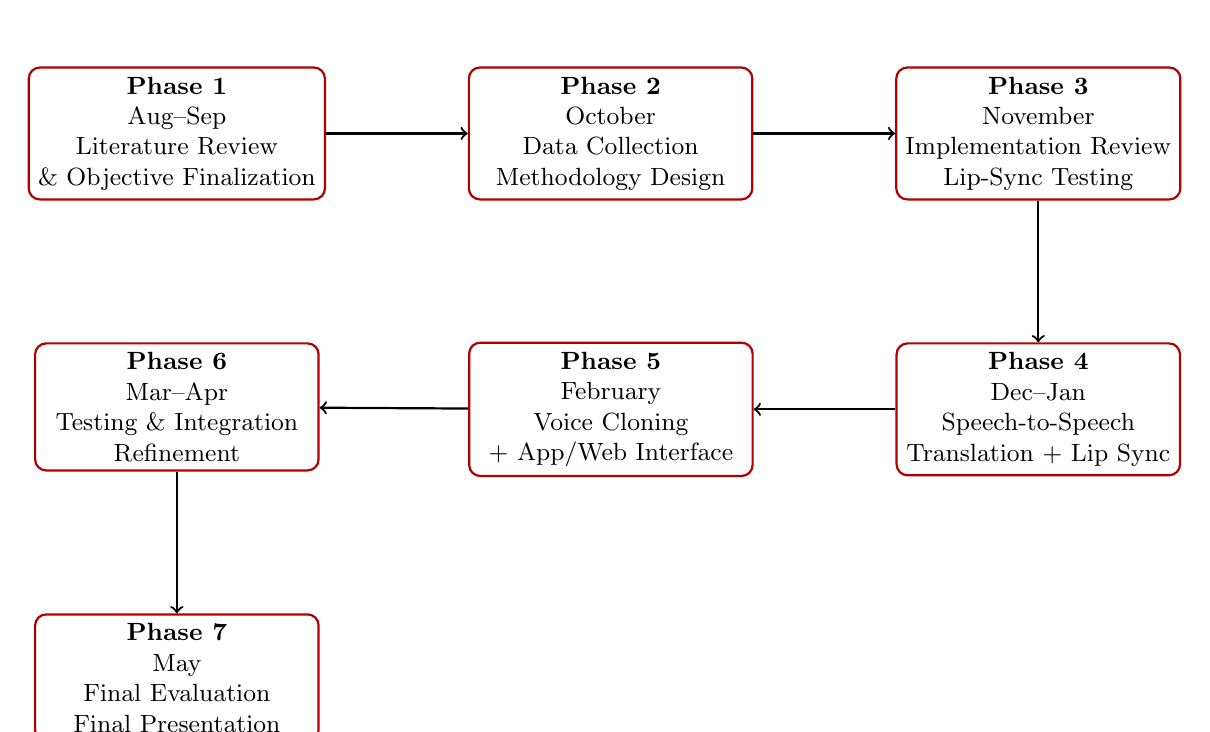
\begin{tikzpicture}[
    node distance=1.8cm,
    box/.style={
        rectangle, rounded corners,
        draw=red!70!black, thick,
        minimum width=3.6cm,
        minimum height=1cm,
        align=center,
        font=\small
    },
    arrow/.style={->, thick}
]

% Nodes
\node[box] (p1) {%
\textbf{Phase 1}\\
Aug--Sep\\
Literature Review\\
\& Objective Finalization
};

\node[box, right=of p1] (p2) {%
\textbf{Phase 2}\\
October\\
Data Collection\\
Methodology Design
};

\node[box, right=of p2] (p3) {%
\textbf{Phase 3}\\
November\\
Implementation Review\\
Lip-Sync Testing
};

\node[box, below=of p3] (p4) {%
\textbf{Phase 4}\\
Dec--Jan\\
Speech-to-Speech\\
Translation + Lip Sync
};

\node[box, left=of p4] (p5) {%
\textbf{Phase 5}\\
February\\
Voice Cloning\\
+ App/Web Interface
};

\node[box, below=1.8cm of p1] (p6) {%
\textbf{Phase 6}\\
Mar--Apr\\
Testing \& Integration\\
Refinement
};

\node[box, below=1.8cm of p6] (p7) {%
\textbf{Phase 7}\\
May\\
Final Evaluation\\
Final Presentation
};

% Arrows
\draw[arrow] (p1) -- (p2);
\draw[arrow] (p2) -- (p3);
\draw[arrow] (p3) -- (p4);
\draw[arrow] (p4) -- (p5);
\draw[arrow] (p5) -- (p6);
\draw[arrow] (p6) -- (p7);

\end{tikzpicture}
\caption{Simplified Block Process Timeline for the Project}
\end{figure}




\section{Contributions}

This work makes the following contributions to the field:

\begin{itemize}
    \item \textbf{First S2ST System for Indian Languages with Cloned Voice:} To our knowledge, this is the first speech-to-speech translation system designed specifically for Indian languages that incorporates personalized voice cloning.
    
    \item \textbf{Integration of Four Advanced AI Models:} Successfully integrated Whisper~\cite{radford2023whisper}, IndicTrans2~\cite{gala2023indictrans2}, IndicF5~\cite{indicf5_2025}, and MuseTalk~\cite{zhang2023musetalk} 1.5 into a cohesive pipeline.
    
    \item \textbf{Custom Dataset Preparation:} Created evaluation datasets for Indian language S2ST assessment.
    
    \item \textbf{Human Evaluation Framework:} Established a human evaluation protocol for assessing subjective quality of the generated outputs.
\end{itemize}

\section{Limitations}

The current system has the following limitations:

\begin{itemize}
    \item \textbf{Lighting Sensitivity:} Lip sync quality varies with lighting conditions and performs suboptimally on low-resolution input videos.
    
    \item \textbf{Accent Similarity:} While accent similarity is high (cosine similarity $\approx$ 0.92), it is not perfect, and some speaker-specific nuances may be lost.
    
    \item \textbf{Long Video Stability:} Long video sequences (beyond 30 seconds) show reduced stability in lip synchronization quality.
    
    \item \textbf{Computational Requirements:} The full pipeline requires significant GPU resources for real-time processing.
    
    \item \textbf{Language Coverage:} Currently supports six Indian languages; many regional languages remain unsupported.
\end{itemize}

\section{Practical Design Takeaways}

Based on the development experience, the following practical insights emerged:
\begin{itemize}
    \item \textbf{Face Preprocessing:} Preprocessing of face frames critically improves lip accuracy. Face detection and alignment should be performed as a preprocessing step.
    
    \item \textbf{Embedding Quality:} Better speaker embeddings directly correlate with better voice similarity. Investment in embedding extraction pays dividends.
    
    \item \textbf{Model Selection:} Whisper~\cite{radford2023whisper} medium model strikes the best balance between speed and accuracy for Indian language ASR.
    
    \item \textbf{Temporal Alignment:} Careful attention to audio-video temporal alignment is essential for natural-looking output.
\end{itemize}

\section{Future Work}

Future development directions include:

\begin{itemize}
    \item \textbf{Extended Language Support:} Expand support to 6+ Indian languages including regional dialects.
    
    \item \textbf{Fine-tuned Lip Motion Dataset:} Create and train on a custom Indian lip-motion dataset for improved performance.
    
    \item \textbf{Custom Voice Encoder:} Train a custom multilingual Indic voice encoder specifically optimized for Indian accents.
    
    \item \textbf{Long-Duration Stability:} Improve stability for long-duration video processing through temporal smoothing techniques.
    
    \item \textbf{Real-time Optimization:} Optimize the pipeline for true real-time processing with reduced latency.
    
    \item \textbf{Mobile/Web Deployment:} Develop lightweight versions suitable for mobile and edge device deployment.
\end{itemize}

\section{Closing Remark}

The developed system represents a significant step toward natural, multilingual AI communication that preserves human identity, clarity, and realism. By integrating state-of-the-art models for ASR, translation, voice cloning, and lip synchronization, this work demonstrates that comprehensive speech-to-speech translation with visual synchronization is not only feasible but can achieve quality levels suitable for practical applications.


\addcontentsline{toc}{chapter}{References}
\nocite{*}
\printbibliography

\end{document}
